\documentclass[a4paper,10pt]{article}
\usepackage[T1]{fontenc}
\usepackage[utf8]{inputenc}
\usepackage{lmodern,textcomp}
\usepackage[margin=2.2cm]{geometry}
\usepackage{amsmath,amssymb,siunitx,booktabs,graphicx,tabularx,array,enumitem,xcolor,fancyhdr,float,fancyvrb}
\usepackage{circuitikz}
\usetikzlibrary{arrows.meta}
\usepackage[colorlinks=true,linkcolor=blue!50!black,urlcolor=blue!50!black]{hyperref}
\setlength{\parindent}{0pt}
\setlength{\parskip}{5pt}
\setlength{\headheight}{14pt}
\renewcommand{\arraystretch}{1.2}
\renewcommand{\tabularxcolumn}[1]{>{\raggedright\arraybackslash}p{#1}}
\setlist{nosep,leftmargin=*}
\newcommand{\file}[1]{\nolinkurl{#1}}
\newcommand{\cmd}[1]{\texttt{#1}}   % for paths and commands with spaces (\nolinkurl drops them)
\newcommand{\todo}[1]{\textcolor{red}{[TODO: #1]}}
\sisetup{per-mode=symbol}
\DeclareSIPrefix\micro{\text{\textmu}}{-6}   % XeTeX (tectonic) otherwise prints a T1 "ţ"
\pagestyle{fancy}\fancyhf{}
\fancyhead[L]{34870 Electroacoustics}
\fancyhead[R]{Loudspeaker project --- System D}
\fancyfoot[L]{Group 10}
\fancyfoot[R]{\thepage}
\graphicspath{{../figures/}{Project/Final design/figures/}{../ltspice/}{Project/Final design/ltspice/}}
% compiles both locally (from Project/Final design/report) and in Overleaf (from the repo root)
\newcommand{\res}[1]{\IfFileExists{#1}{\input{#1}}{\input{Project/Final design/report/#1}}}
\newcommand{\verbfile}[1]{\IfFileExists{../data/dsp/#1}{\VerbatimInput[fontsize=\footnotesize]{../data/dsp/#1}}{\VerbatimInput[fontsize=\footnotesize]{"Project/Final design/data/dsp/#1"}}}
\res{results_task1.tex}
\res{results_design.tex}
\newenvironment{idea}{\par\smallskip\noindent\begin{minipage}{\linewidth}\small\color{blue!35!black}\textbf{The idea in one line:}\ }{\end{minipage}\par\smallskip}

\begin{document}
\begin{center}
{\Large\bfseries Loudspeaker project --- three-way System D}\\[5pt]
{\large How we designed it, step by step}\\[5pt]
34870 Electroacoustics · Group 10: Louis Andrianne, Sophie Kimura, Mads Rudolph\\[4pt]
System D (shared with Group 4): Scan-Speak 26W/8534G00 woofer box + DALI Spektor 2 (S/N 7446912 -- L)
\end{center}
\thispagestyle{fancy}

\begin{center}
\fbox{\begin{minipage}{0.92\linewidth}\small
\textbf{What this document is.} It is not the hand-in. It is our own explanation of the design: what
we simulated, how each simulation works, why we ended up with these values, and how to put the
MiniDSP and the filter board together. Tasks 1 and 2 are done in simulation; Tasks 3 and 4 are
prepared and wait for lab time. Every number in the text is written by the scripts
(\file{results_task1.tex}, \file{results_design.tex}), so if the design changes and the scripts are
rerun, the text follows. How to rerun everything: \cmd{Project/Final design/README.md}.
\end{minipage}}
\end{center}

\tableofcontents
\newpage

% =====================================================================================
\section{What we are building}

A single loudspeaker driver cannot play the whole audio range well. A big cone moves enough air for
bass but becomes directional and starts to break up at high frequencies; a small dome is the other
way round. System D therefore has three drivers, and our job is to decide \emph{which driver plays
which frequencies}, and to make the three of them add up to one smooth response.

\begin{center}
\begin{tabularx}{\linewidth}{lXl}
\toprule
Driver & What it is & What it should play \\
\midrule
Woofer & Scan-Speak 26W/8534G00, \SI{26}{cm} cone, in an \SI{88}{L} box with vents & the bass, up to about \SI{\xxWM}{Hz} \\
Midrange & DALI Spektor 2, 5\textonequarter\,in cone, closed box & about \SI{\xxWM}{Hz} to \SI{\xxMT}{Hz} \\
Tweeter & DALI Spektor 2, \SI{25}{mm} soft dome & everything above about \SI{\xxMT}{Hz} \\
\bottomrule
\end{tabularx}
\end{center}

The frequency where one driver hands over to the next is a \textbf{crossover frequency}. We have two.
The project guide fixes \emph{how} each one is made (Figure~\ref{fig:xcircuit}):
\begin{itemize}
\item \textbf{Woofer $\leftrightarrow$ midrange: digital.} The MiniDSP is a small computer that
  filters the music before the amplifier. Output~1 keeps only the bass and goes through amplifier
  channel~1 straight to the woofer. Output~2 keeps everything above the bass and goes through
  amplifier channel~2.
\item \textbf{Midrange $\leftrightarrow$ tweeter: passive.} The signal from amplifier channel~2 goes
  into a board with coils, capacitors and resistors. A coil lets low frequencies through and blocks
  high ones, a capacitor does the opposite. That board splits the signal once more between midrange
  and tweeter.
\end{itemize}

\res{crossover_circuit.tex}

\textbf{Our final design in one table.} The rest of the document explains where each line comes from.
\begin{center}
\begin{tabular}{ll}
\toprule
Woofer box & one vent open, length $L = \SI{160}{mm}$, box tuned to $f_B = \SI{\bfBA}{Hz}$, no extra filling \\
Digital crossover & \xalignDig\ (Linkwitz--Riley, 4th order) at \SI{\xfcDig}{Hz}; woofer turned down \SI{\xgWoof}{dB} \\
Midrange filter & 2nd-order low-pass: coil \xMidLa\ in series, capacitor \xMidCa\ across the driver \\
Tweeter filter & 2nd-order high-pass: capacitor \xTwCa\ in series, coil \xTwLa\ across; \\
 & then an L-pad: \xTwRs\ in series, \xTwRp\ across the tweeter \\
Wiring & all three drivers normal polarity (red to $+$) \\
Result (simulated) & from \SI{150}{Hz} to \SI{15}{kHz} within \SI{\xspreadOn}{dB} straight in front, \SI{\xspreadOff}{dB} at $30^\circ$ \\
\bottomrule
\end{tabular}
\end{center}

\subsection{Words we use a lot}
\begin{description}[leftmargin=2.4cm,labelwidth=2.2cm,style=sameline]
\item[$p/V$] Sound pressure the speaker produces per volt from the amplifier. Our ``response''. In dB
  re \SI{1}{Pa/V}.
\item[Phase] How far a signal is shifted in time, as an angle. Two drivers playing the same
  frequency add up fully when their phases match (\SI{0}{\degree} apart) and cancel when they are
  \SI{180}{\degree} apart. This is why every response here has a phase plot.
\item[$Z_i$] The driver's input impedance: what the amplifier ``sees'' when it pushes current into
  the driver. It is not a constant resistance; it changes with frequency.
\item[$f_B$, $f_3$] Box tuning frequency (where the vent does most of the work) and the
  frequency where the bass has dropped \SI{3}{dB}, our measure of how deep the speaker plays.
\item[Order] How steep a filter is. 2nd order falls \SI{12}{dB} per octave, 4th order \SI{24}{dB}.
\end{description}

% =====================================================================================
\section{What we measured, and what each measurement is used for}

Everything is built on our own measurements of the actual units, not on data sheets. That is the
point of the project: a driver in the lab differs from its data sheet, and the box and the room add
their own effects.

\begin{center}
\begin{tabularx}{\linewidth}{lXX}
\toprule
Measurement & What it tells us & Where we use it \\
\midrule
Lab D: woofer impedance, free air and in the closed box & the driver's mechanical properties (how heavy, how stiff, how strong the motor is) & Task 1: the values in the box circuit \\
Lab D: woofer impedance with one vent at 160/200/240 mm & how the vent changes the box & Task 1: the vent's air mass \\
Lab D: near-field pressure at cone and vent & how loud cone and vent really are at low frequencies & Task 1: checking the box circuit \\
Lab D: midrange and tweeter impedance $Z_i$ & the load the passive filters drive & Task 2: loading the filters correctly \\
Lab E: $p/V$ of all three units, straight on and at $30^\circ$ & what each driver sounds like in its box, magnitude and phase & Task 2: the drivers in the crossover simulation \\
\bottomrule
\end{tabularx}
\end{center}

Two limits to keep in mind. The anechoic chamber (Lab E) only works above about \SI{125}{Hz}, and
Lab E was measured with the woofer vents plugged. So the Lab E data says nothing useful about the
bass. That is why Task 1 (bass) and Task 2 (everything else) are two separate simulations, which we
join at the end.

% =====================================================================================
\section{Task 1: tuning the woofer box}

\subsection{What we can change}
The box is already built (\SI{88}{L}), so we cannot pick its size. What we can change is:
\begin{itemize}
\item \textbf{the vents:} the box has two telescopic tubes. We can plug both (a closed box), open one,
  or open both, and slide the tube in or out to change its length;
\item \textbf{filling:} damping wool inside makes the box act slightly larger.
\end{itemize}
To compare these options we need a model, because the chamber cannot measure the bass and tuning
by ear is unreliable.

\subsection{How a vented box works}
Think of the air in the box as a spring and the air plug inside the vent tube as a small mass sitting
on that spring. Like any mass on a spring, it has one frequency where it bounces easily: the box
tuning frequency $f_B$. Around $f_B$ the cone pushes on the box air, the air plug in the vent moves
a lot, and \emph{the vent} radiates most of the sound while the cone itself hardly moves. Above
$f_B$ the vent's air plug is too heavy to follow and the cone takes over. Below $f_B$ the vent and the
cone move in opposite directions and cancel each other, so the bass falls off steeply.

A longer or narrower vent has a heavier air plug, so $f_B$ goes down. Two vents open side by side act
like two masses next to each other: the air has two ways out, the total mass is smaller, and $f_B$
goes up.

\subsection{The circuit}
We draw the woofer and box as an electrical circuit in LTspice (Figure~\ref{fig:task1sch}). This is
the analogy method from Lectures 7 and 8: in every part of the system something pushes and something
flows, and we write both as a voltage and a current.
\begin{center}
\begin{tabularx}{\linewidth}{lllX}
\toprule
Part & ``Voltage'' & ``Current'' & Elements and what they physically are \\
\midrule
Electrical & voltage & current & $R_E$ the coil's resistance, $L_E$ the coil's inductance \\
Mechanical & force & cone velocity & $M_{MD}$ the cone's mass, $C_{MS}$ the suspension's softness, $R_{MS}$ its friction \\
Acoustical & pressure & air flow (volume velocity) & $C_{AB}$ the box air (the spring), $M_{AP}$ the vent's air plug, $R_{AP}$, $R_{AL}$ losses in the vent and leaks, and the air in front of the cone (radiation impedance) \\
\bottomrule
\end{tabularx}
\end{center}
The parts are linked by the motor: current in the coil gives a force $F = Bl\,i$, and a moving coil
gives a voltage back, $e = Bl\,u$. The cone turns velocity into air flow by its area $S_D$.

LTspice then solves the circuit at each frequency. From the result we read the air flow out of the
cone, $U_D$, and out of the vent, $U_P$. The pressure \SI{1}{m} away (speaker on the floor, so sound
goes into a half space) is
\[ p = j\omega\rho\,\frac{U_D - U_P}{2\pi r}. \]
The minus sign is there because the vent flow is counted into the box; the vent breathes out when the
cone moves in.

\subsection{Getting the values: fitting the circuit to the impedance}
The circuit is only as good as its values. The data sheet gives a set, but our driver is not exactly
the data-sheet driver. So we got the values from our own Lab D impedance curves by \emph{fitting}.

The impedance is a good fingerprint of the driver. Its peak sits at the resonance, and its height and
width tell how much damping there is. Fitting means: guess all the unknown values, let the circuit
compute its impedance, compare it with the measured curve (magnitude and phase), adjust the values,
and repeat until the two curves lie on top of each other. The computer does the adjusting (a
standard search method called Nelder--Mead).

We fitted the free-air curve and the closed-box curve at the same time. Free air alone cannot tell the
cone's mass from its stiffness. The closed box adds a known spring (the box air,
$C_{AB} = V_B/\rho c^2$), which moves the resonance up, and from that shift both are pinned down.
$R_E = \SI{5.7}{\ohm}$ was measured with a multimeter and $S_D$ was taken from the data sheet.

\begin{center}
\begin{tabular}{lccc}
\toprule
 & Lab D, read off & Lab D, fit & Data sheet$^\ast$ \\
\midrule
$f_S$ (Hz), driver resonance & 22.7 & \bfS & 22.9 \\
$Q_{MS}$ (mechanical damping) & 9.95 & \bQMS & 9.1 \\
$Q_{ES}$ (electrical damping) & 0.511 & \bQES & 0.41 \\
$Q_{TS}$ (total) & 0.486 & \bQTS & 0.39 \\
$V_{AS}$ (L), suspension softness as air volume & 213 & \bVAS & 165 \\
$Bl$ (T\,m) & -- & \bBl & 10.1 \\
$M_{MS}$ (g) & -- & \bMMS & 50.5 \\
$C_{MS}$ (mm/N) & -- & \bCMS & 0.95 \\
$R_E$ ($\Omega$), $L_E$ (mH) & 5.7, -- & 5.7, \bLE & 5.7, -- \\
\bottomrule
\end{tabular}\\[2pt]
{\footnotesize $^\ast$ $f_S$, $Q$s and $V_{AS}$ computed from the data sheet's $M_{MS}$, $C_{MS}$, $Bl$, $R_{MS}$ and $S_D = \SI{350}{cm^2}$.}
\end{center}

Our driver is softer than the data sheet says ($V_{AS}$ about 25\,\% larger) and has a weaker motor
($Q_{ES}$ 0.50 instead of 0.41). Both are normal for a used driver from a different batch. If we had
used the data sheet, every tuning below would have been off. Figure~\ref{fig:zfit} shows that the
fitted circuit reproduces the measured curves.

\begin{figure}[htbp]
\centering
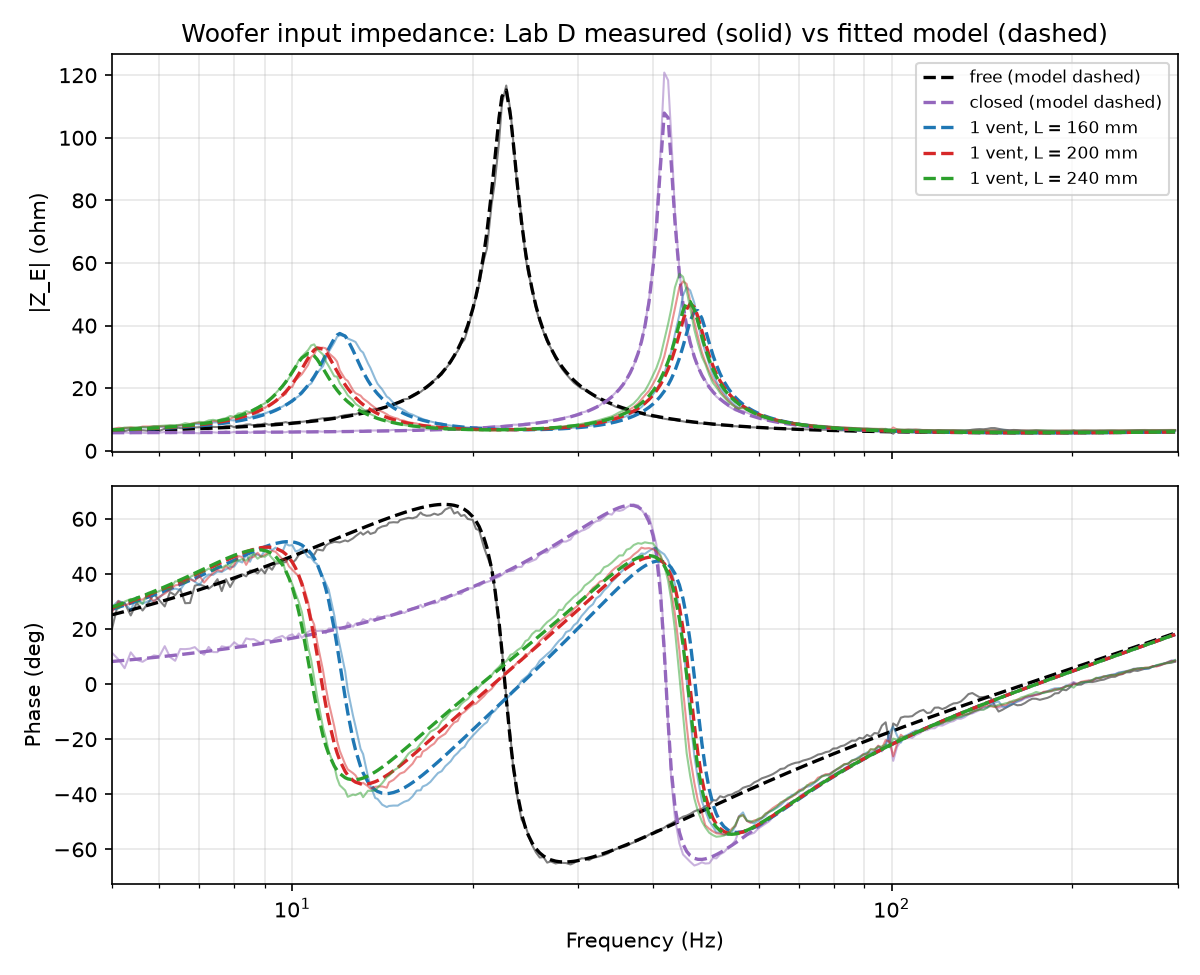
\includegraphics[width=0.82\linewidth]{task1_impedance_fit.png}
\caption{Woofer impedance, Lab D measured (thin lines) and our fitted circuit (dashed), magnitude and
phase. Free air (black): one peak at $f_S$. Closed box (purple): one peak, higher, because the box air
stiffens the cone. Vented (coloured): two peaks; the dip between them is $f_B$, and it moves down as
the vent gets longer.}\label{fig:zfit}
\end{figure}

\subsection{The vent's air mass}
With the driver known, the three vented impedance curves give the vent. The textbook formula for the
air plug's mass is $M_{AP} = \rho(L + 1.46a)/\pi a^2$, with $L$ the tube length and $a$ its radius
(\SI{32.5}{mm}). The measurement did not follow it: from $L = 160$ to \SI{240}{mm}, $f_B$ moved only
half as much as the formula predicts. So instead of trusting the formula we fitted one mass for each
length we measured:
\begin{center}
\begin{tabular}{lccc}
\toprule
Vent length & $M_{AP}$ fitted (kg/m$^4$) & $M_{AP}$ formula & $f_B$ (Hz) \\
\midrule
\SI{160}{mm} & \bMAPA & \bMAPformulaA & \bfBA \\
\SI{200}{mm} & \bMAPB & \bMAPformulaB & \bfBB \\
\SI{240}{mm} & \bMAPC & \bMAPformulaC & \bfBC \\
\bottomrule
\end{tabular}
\end{center}
The likely reason is that the length we wrote down is how far the telescope was pulled out, not the
length the air actually sees, or that the inner tube is narrower than \SI{65}{mm}.
\todo{measure both vents' inner diameters and the telescope range on the box.}

A second thing the fit showed: with the vents plugged the box has almost no losses (the closed-box
peak reaches \SI{121}{\ohm}), but with a vent open the curves need extra losses
($Q_L = \bQL$, $Q_P = \bQP$). The losses come from the air rushing through the vent, not from leaks in
the box. So the model uses different losses for the plugged and the vented box.

\subsection{Checking the model against the near field}
Fitting the impedance only proves the circuit gets the \emph{electrical} side right. To check that
it also gets the \emph{sound} right, we compare it with the Lab D near-field measurements: a
microphone almost touching the cone, and one at the vent opening. Very close to a source, the
pressure is simply proportional to the air flow through it, $p \approx j\omega\rho\,U/\pi a$, so the
circuit can predict exactly what those microphones should read.

Nothing in Figure~\ref{fig:nf} is fitted; it is a pure prediction. Cone and vent agree within
2--3\,dB, they cross where the measurement crosses, and the cone has its dip right at $f_B$. That is
the cone ``resting'' while the vent plays, and it confirms the model. Two differences are not the
model's fault. Above about \SI{60}{Hz} the vent microphone also picks up the cone, so the measured
vent curve stops falling. Below \SI{120}{Hz} the room (026) adds ripple from its own resonances.

\begin{figure}[htbp]
\centering
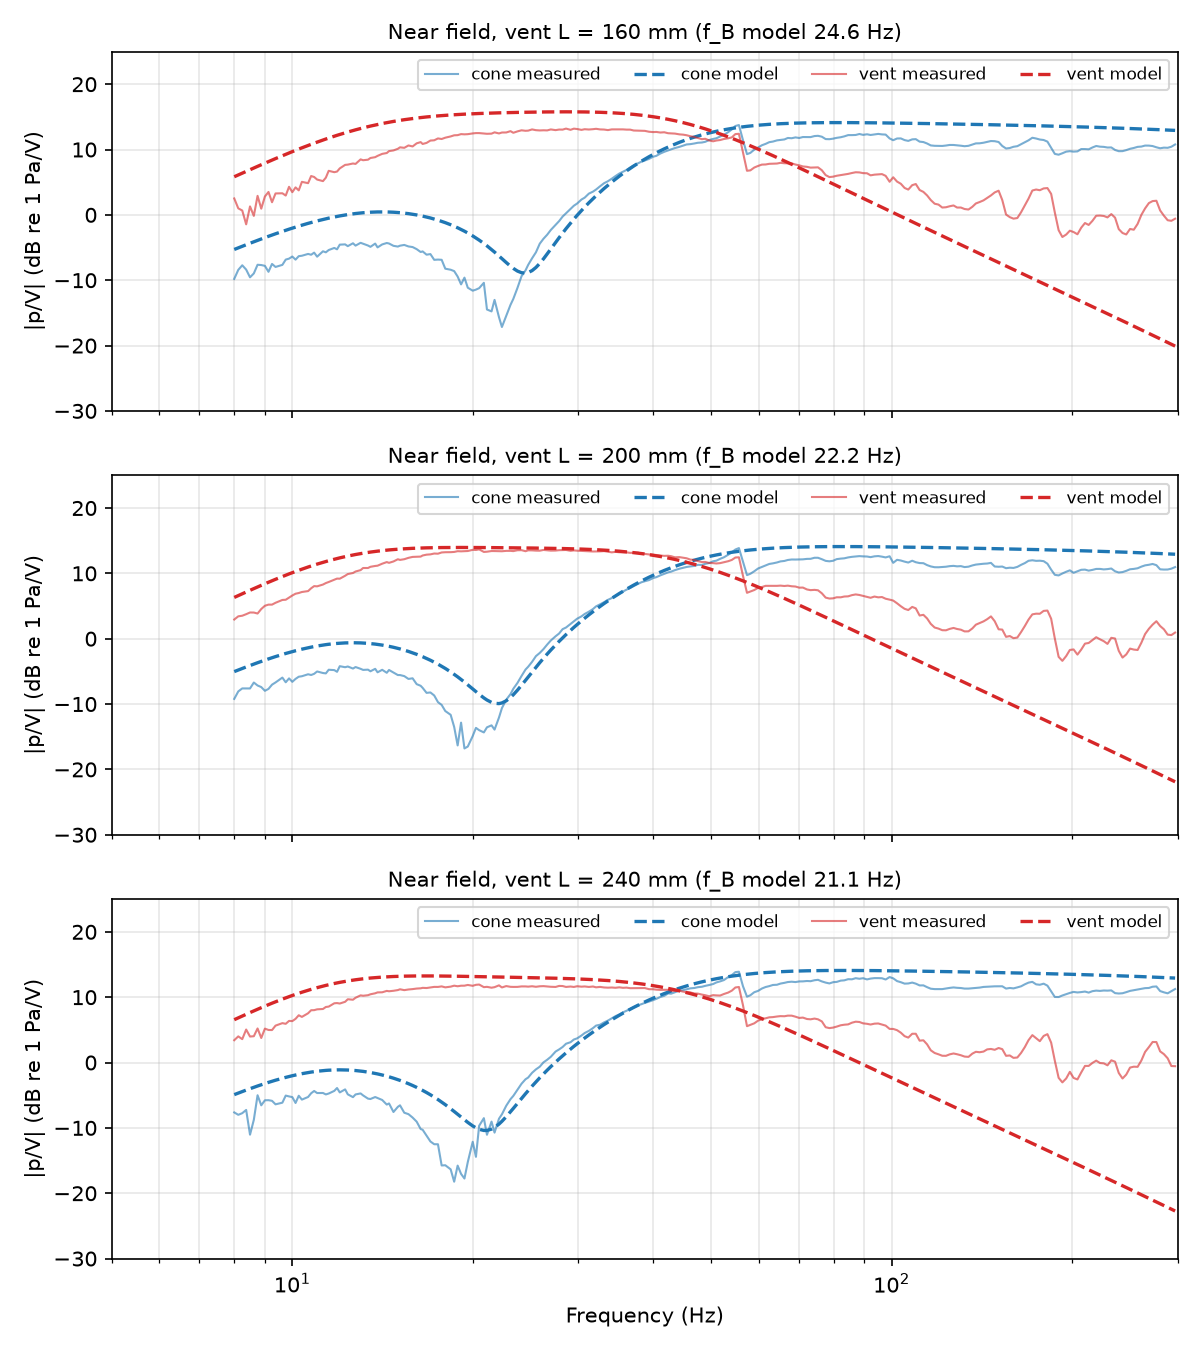
\includegraphics[width=0.8\linewidth]{task1_nearfield.png}
\caption{Near-field pressure at the cone (blue) and at the vent (red), measured in Lab D (thin) and
predicted by the circuit (dashed), for the three vent lengths. Predicted, not fitted.}\label{fig:nf}
\end{figure}

\subsection{Trying the options and choosing one}
With a model we trust, we tried every option in LTspice. One run with \file{.step} goes through the
plugged box, the three vent lengths, and a free value for experimenting
(Figure~\ref{fig:task1sch}). Figure~\ref{fig:tuning} shows the result.

\begin{center}
\begin{tabular}{lccc}
\toprule
Configuration & $f_B$ (Hz) & $f_3$ (Hz) & ripple (dB) \\
\midrule
Vents plugged (closed box) & -- & \bfthreeCl & \brippleCl \\
One vent, $L = \SI{160}{mm}$ & \bfBA & \bfthreeA & \brippleA \\
One vent, $L = \SI{200}{mm}$ & \bfBB & \bfthreeB & \brippleB \\
One vent, $L = \SI{240}{mm}$ & \bfBC & \bfthreeC & \brippleC \\
Both vents ($M_{AP} \approx 52$) & 28.0 & 32.7 & +2.4 \\
\bottomrule
\end{tabular}\\[2pt]
{\footnotesize $f_3$ relative to the average level at \SIrange{150}{300}{Hz}, half space, no room. Ripple = how far the response rises above that level below \SI{150}{Hz} (a ``hump'').}
\end{center}

How to read it:
\begin{itemize}
\item Opening a vent gains about \SI{4}{Hz} of bass ($f_3$ 37 $\to$ \SI{33}{Hz}) at the cost of a
  small hump.
\item Once a vent is open, \emph{the length hardly matters for $f_3$}: every $f_B$ from 21 to
  \SI{28}{Hz} gives about \SI{33}{Hz}. Only the hump changes. This is because our driver is very soft
  compared with the box ($V_{AS}$ is 2.3 times $V_B$). The standard alignments from Lecture~8 (QB3,
  B4, C4) assume a specific ratio, so none of them can be reached with this box; the guide says the same.
\item The lower plot shows how far the cone moves. Between 25 and \SI{40}{Hz} the vented cone moves a
  third as much as the closed one, so it can play louder before it distorts.
\end{itemize}

\textbf{Choice: one vent at \SI{160}{mm}.} It gives the same $f_3$ as the longer settings, cuts the
cone excursion, and it is a setting we actually measured, so the near field checks it directly.
Opening both vents gives no deeper bass and a bigger hump. Filling would add a few hertz, but we have no
measurement with filling to check the model against. A room adds bass of its own, so a hump under
\SI{2}{dB} in this free-space model is on the safe side.

\begin{figure}[htbp]
\centering
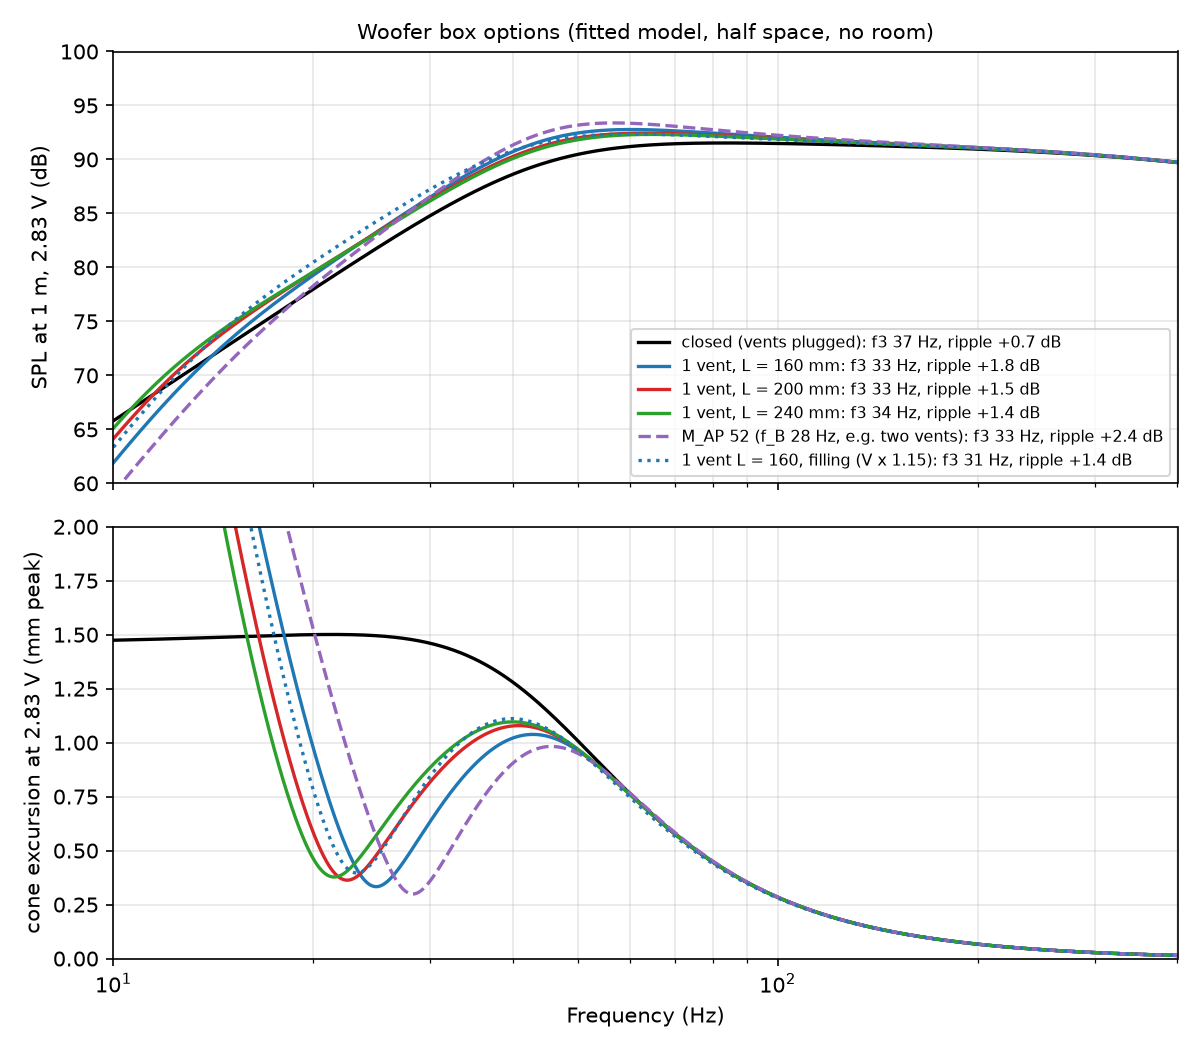
\includegraphics[width=0.8\linewidth]{task1_tuning.png}
\caption{All options at \SI{2.83}{V}, \SI{1}{m}, half space. Top: sound pressure level. Bottom: how far
the cone moves. Note the vented cone's dip at $f_B$: the vent does the work there.}\label{fig:tuning}
\end{figure}

\begin{figure}[htbp]
\centering
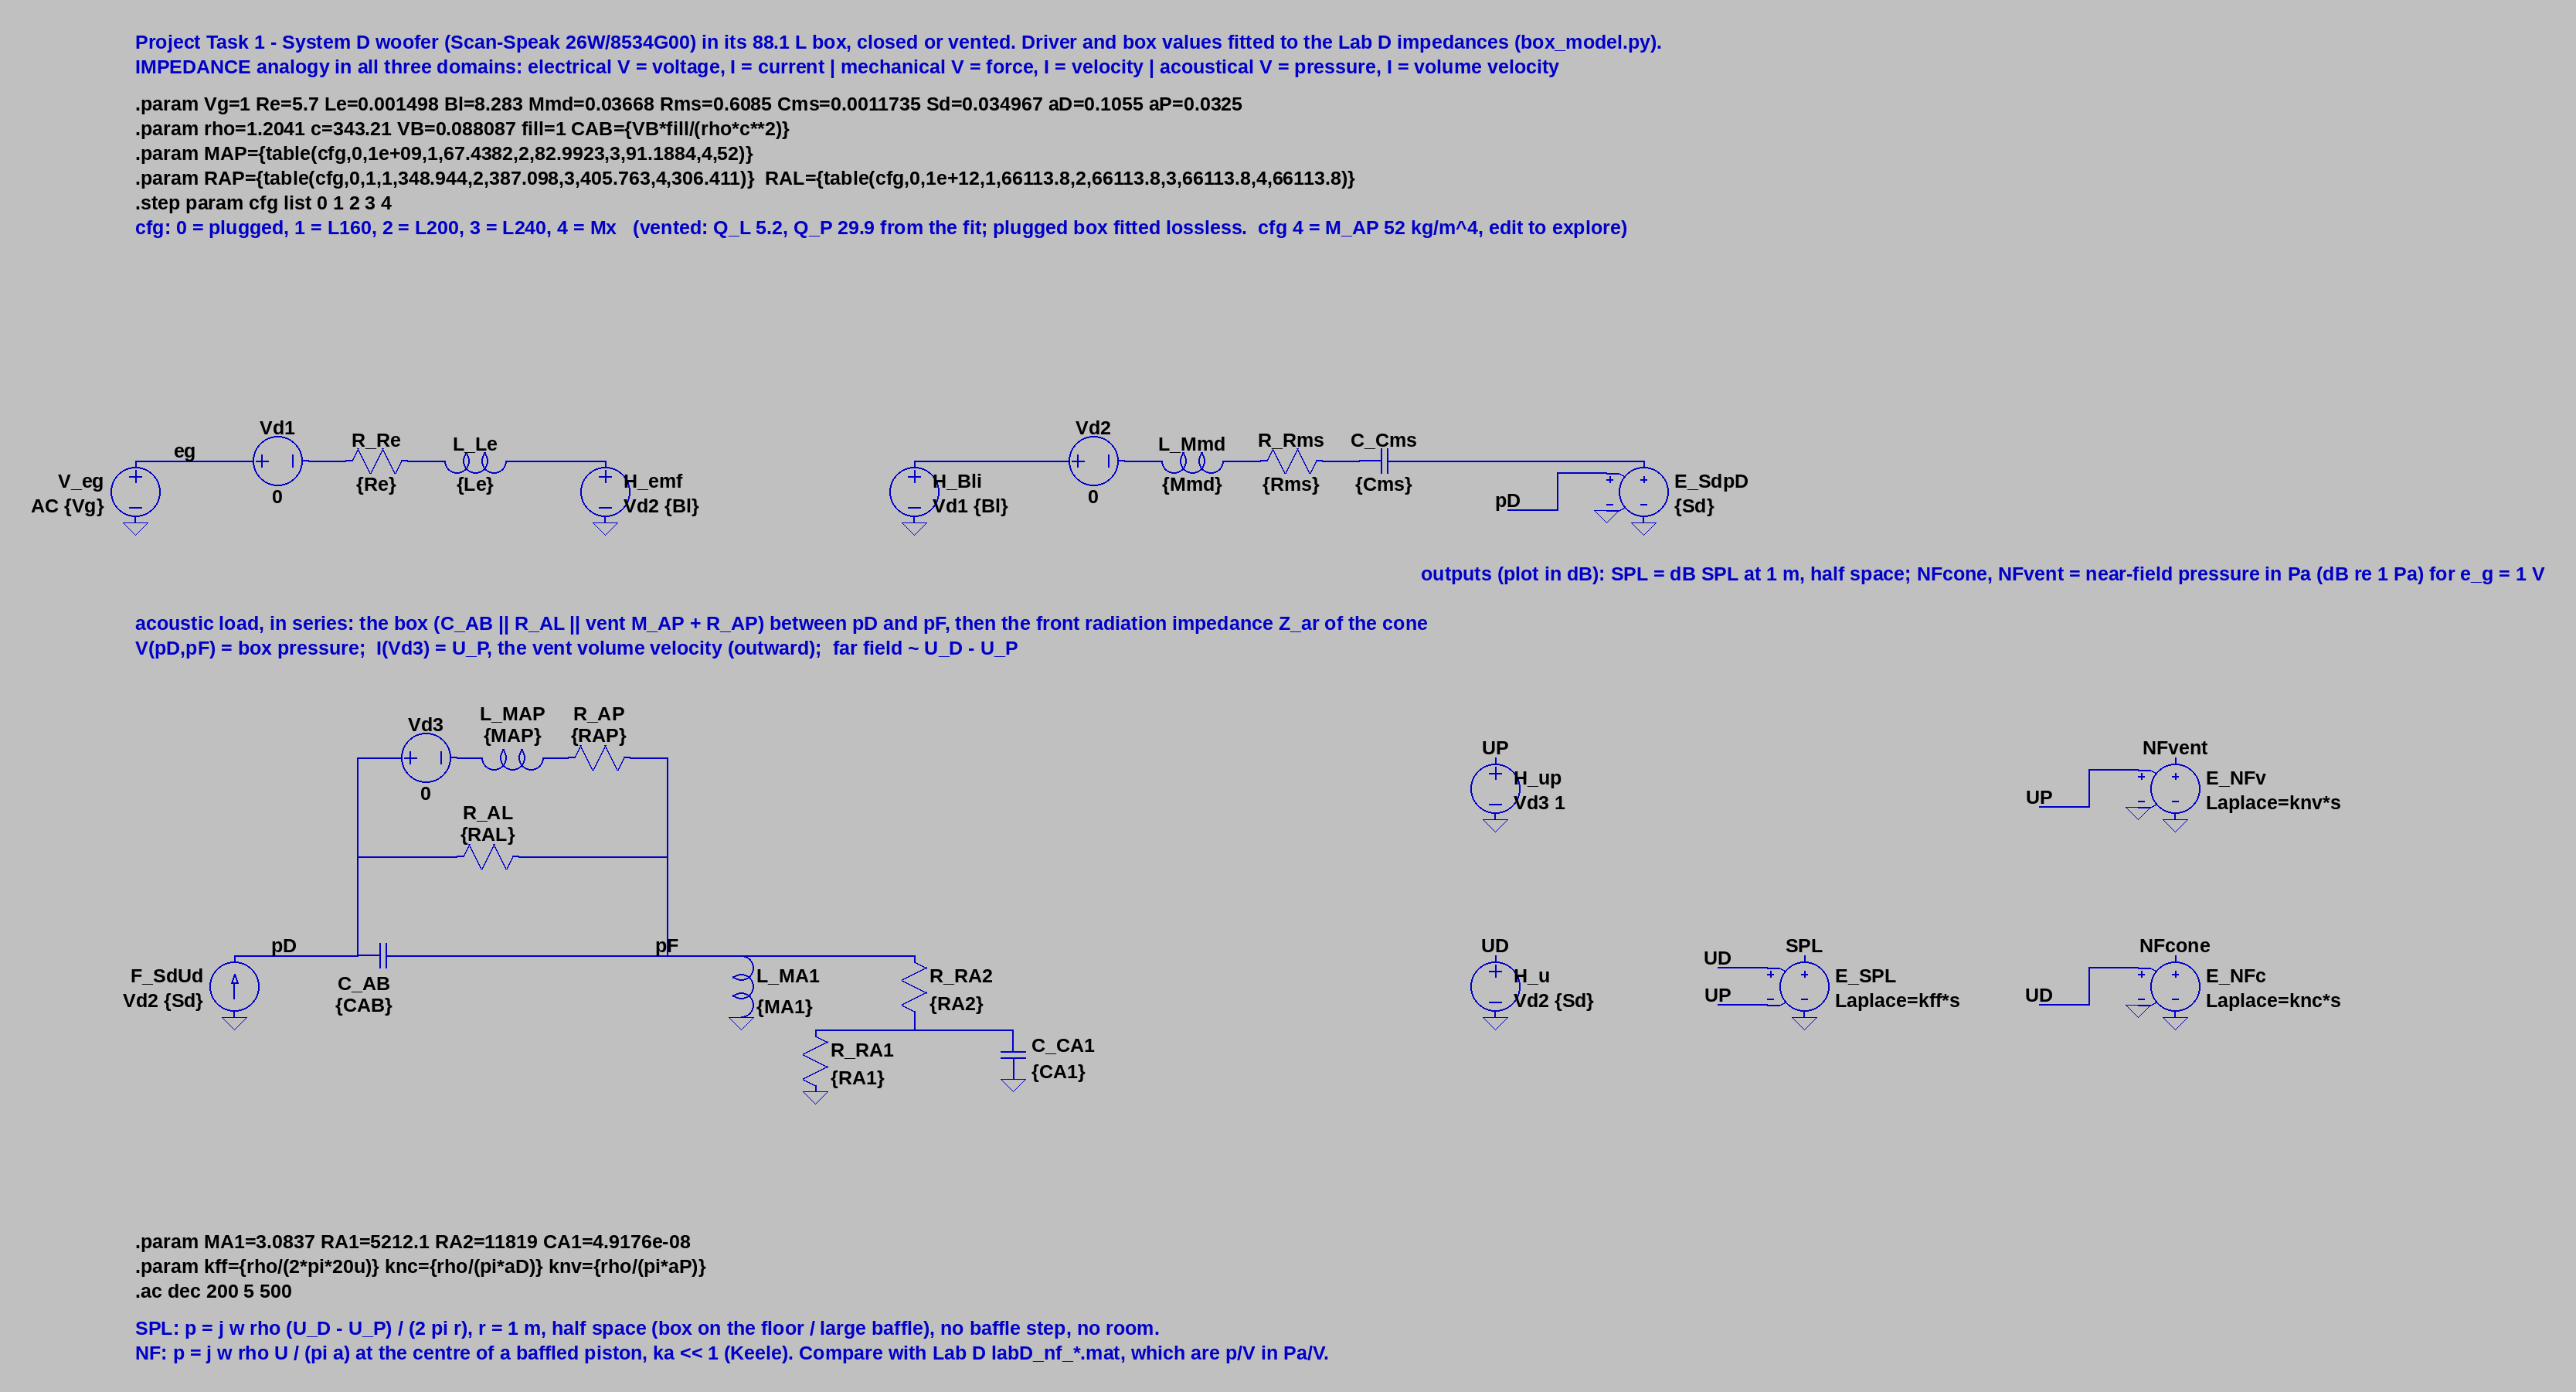
\includegraphics[width=\linewidth]{task1/preview/Task1_WooferBox.png}
\caption{\file{ltspice/task1/Task1_WooferBox.asc}. Top row: electrical part ($R_E$, $L_E$, the back
voltage $Bl\,u$) and mechanical part (force $Bl\,i$, cone mass, friction, suspension). Bottom: the
acoustic part. The cone's air flow enters at \file{pD}, splits between the box air $C_{AB}$, the leak
$R_{AL}$ and the vent ($M_{AP}$, $R_{AP}$), and leaves through the air in front of the cone. The sources on
the right turn the flows into far-field and near-field pressure. \file{cfg} selects plugged / 160 / 200
/ 240\,mm.}\label{fig:task1sch}
\end{figure}

% =====================================================================================
\section{Task 2: designing the crossover}

\subsection{What a crossover has to do}
Each filter only has to do something simple: let one band through and attenuate the rest. The hard
part is the \emph{overlap}. Around each crossover frequency two drivers play at the same time, and the
listener hears their \emph{sum}. How they add depends on their phase:
\begin{center}
\begin{tabular}{lcc}
\toprule
Two equal signals that are & sum compared with one of them & sum compared with the ``power sum'' \\
\midrule
in phase (\SI{0}{\degree} apart) & $+6$\,dB & $+3$\,dB \\
\SI{90}{\degree} apart & $+3$\,dB & $0$\,dB \\
\SI{180}{\degree} apart & they cancel & $-\infty$ \\
\bottomrule
\end{tabular}
\end{center}
The phase of each driver's output is the filter's phase \emph{plus} the driver's own phase \emph{plus}
the delay from where it sits on the box. So the filter cannot be chosen from a textbook alone. We have
to simulate the real drivers. The ``power sum'' (adding the energies and ignoring phase) is a handy
reference: if the real sum lies \SI{3}{dB} above it at a crossover, the two drivers are in phase there;
if it falls below, they are cancelling.

\subsection{Getting the real drivers into LTspice}
The course script \file{Matlab2LTspice.m} turns a measured curve into a text file that LTspice can
load with \file{.inc}. Each file defines a special voltage or current source that, at every
frequency, follows a table of the measured magnitude and phase. Per driver there are two:
\begin{itemize}
\item \textbf{the response ($TF$):} a voltage source that outputs $V(\mathrm{Pout}) = TF(f)\cdot
  V(\mathrm{Vspkr})$. Put the voltage that reaches the driver in, and the sound pressure the driver
  would make comes out (as a voltage, 1~V = 1~Pa). The data is Lab E's $p/V$ at the microphone,
  \SI{2.44}{m} away.
\item \textbf{the impedance ($Z_i$, midrange and tweeter only):} a current source that draws
  $I = V/Z_i(f)$ from the filter. To the filter it looks exactly like the real driver connected to it.
  The woofer does not need one, because nothing sits between the amplifier and the woofer, and an
  amplifier output keeps its voltage whatever the load.
\end{itemize}
We checked each unit alone first (\file{ltspice/units/Unit_*.asc}): LTspice gives back the measured
$Z_i$ and $p/V$ to within \SI{0.04}{dB}.

\textbf{The distance correction.} Sound takes \SI{7}{ms} to travel \SI{2.44}{m}, and at high
frequencies that delay turns the measured phase into a fast spin that is impossible to read.
\file{Matlab2LTspice.m} removes most of it by multiplying with $e^{+jkd}$, that is, by
undoing the delay of a distance $d$. We used $d = \SI{-1.15}{m}$ (chosen in Lab E so the curves read
well) and, importantly, \emph{the same $d$ for all three drivers}. The three were measured in one run
from one microphone position, so the differences in their phase are real: they come from the
drivers sitting at different places on the box. A separate $d$ per driver would erase exactly the
information the crossover depends on. The impedances are not corrected at all, because no sound
travels anywhere in an impedance measurement.

\subsection{Choosing the two crossover frequencies}
Before any filter, the drivers themselves tell us roughly where to cross:
\begin{itemize}
\item \textbf{Woofer to midrange, \SIrange{300}{400}{Hz}.} The woofer cone is big. At about
  \SI{520}{Hz} its size equals the wavelength divided by $2\pi$ ($ka = 1$), and above that it beams
  its sound forward; above \SI{1.5}{kHz} the cone breaks up and the $30^\circ$ curve falls apart. So it
  should hand over well before that. The midrange has its resonance at \SI{90}{Hz} and is flat from
  about \SI{150}{Hz}, so it can take over from about \SI{300}{Hz}.
\item \textbf{Midrange to tweeter, \SIrange{2.5}{4}{kHz}.} The tweeter has its resonance at
  \SI{1.45}{kHz}. A small dome pushed hard at or below its resonance moves a lot and distorts, and its
  impedance peaks there, which disturbs a passive filter (Section~\ref{sec:zrule}). So the tweeter
  crossover must sit well above \SI{1.45}{kHz}. The midrange is still well behaved at $30^\circ$ up to
  about \SI{4}{kHz}.
\item \textbf{Levels.} In Lab E the woofer is about \SI{4}{dB} louder per volt than the midrange, and
  the tweeter about \SIrange{8}{10}{dB} louder. Both have to be brought down to the midrange's level.
\end{itemize}

\subsection{The digital filter (woofer and midrange)}\label{sec:dsp}
\textbf{What the MiniDSP does.} It samples the music \num{96000} times a second ($f_s = \SI{96}{kHz}$).
A \emph{biquad} is the basic filter block: each new output sample is a weighted sum of the newest two
input samples, the one before, and the last two output samples,
\[
y[n] = b_0\,x[n] + b_1\,x[n-1] + b_2\,x[n-2] + a_1\,y[n-1] + a_2\,y[n-2].
\]
Five numbers ($b_0, b_1, b_2, a_1, a_2$) decide whether it is a low-pass or high-pass, where its
corner is and how sharp it bends (its $Q$). Two biquads in a row give a 4th-order filter.

\textbf{Why Linkwitz--Riley 4 (LR4).} We tried three types (Figure~\ref{fig:phase}):
\begin{itemize}
\item \textbf{Butterworth 2 (BW2):} the low-pass and the high-pass come out \SI{180}{\degree} apart,
  so one driver must be wired inverted, and then they still add to a \SI{3}{dB} bump at the crossover.
\item \textbf{Butterworth 4 (BW4):} the course script's $n = 4$. Its outputs are \SI{360}{\degree}
  apart (in phase again) but each is only \SI{3}{dB} down at the crossover, so they add to a
  \SI{3}{dB} bump.
\item \textbf{Linkwitz--Riley 4 (LR4):} each output is \SI{6}{dB} down at the crossover and the two are
  in phase at \emph{every} frequency. Two halves in phase add back to exactly the original: a flat
  sum, no bump, normal polarity. This won.
\end{itemize}
An LR4 is two identical Butterworth 2nd-order biquads in a row ($Q = 0.707$ each). The course script
\file{DigitalCrossover.m} only makes Butterworth filters, so we ran it with $n = 2$ (one BW2 biquad) and
used the same biquad twice. Our own script does the same thing (the \file{bq} function in
\file{design/xover.py} is a copy of the script's \file{BQ}), and the numbers are identical.

\textbf{The digital filter in LTspice.} LTspice cannot run a sampled filter, but it can use
$e^{-sT}$, which is a delay of exactly one sample ($T = 1/f_s = \SI{10.4}{\micro s}$). Writing the
biquad with $e^{-sT}$ in place of each ``previous sample'' gives a \file{Laplace=} string for an E
source that behaves exactly like the MiniDSP. Two E sources in a row make the LR4.

\textbf{The woofer level.} Output~1's gain is \SI{\xgWoof}{dB}, which matches the woofer's extra
sensitivity. It costs nothing in a digital crossover, because each output has its own amplifier
channel. (Turning the woofer down with resistors would spoil the box tuning, Lecture~9.)

\subsection{The passive filters (midrange and tweeter)}
\textbf{Starting point: the textbook.} A 2nd-order low-pass is a coil in series and a capacitor
across the driver: at high frequencies the coil blocks and the capacitor shorts what gets through. A
2nd-order high-pass is the mirror image, a capacitor in series and a coil across. The Lecture~9
formulas, assuming the driver is a plain resistor $R_E$, give for a Butterworth at \SI{\xxMT}{Hz}:
\begin{center}
\begin{tabular}{lll}
\toprule
 & textbook (driver = resistor) & what we chose \\
\midrule
midrange low-pass, $R_E \approx \SI{5}{\ohm}$ & $L = \SI{0.30}{mH}$, $C = \SI{6.0}{\micro F}$ & \xMidLa, \xMidCa \\
tweeter high-pass, $R_E \approx \SI{3.6}{\ohm}$ & $C = \SI{8.3}{\micro F}$, $L = \SI{0.22}{mH}$ & \xTwCa, \xTwLa, + L-pad \\
\bottomrule
\end{tabular}
\end{center}
The midrange values differ a lot from the textbook. That is not a mistake; the next section explains why.

\subsection{The impedance rule (Lecture 9)}\label{sec:zrule}
A passive filter is a voltage divider between its parts and the driver, so what comes out depends
on the driver's impedance. The textbook assumes a constant resistor. A real driver is not one:
\begin{itemize}
\item \textbf{Midrange:} the voice coil is a coil, so the impedance rises with frequency: \SI{5}{\ohm}
  at \SI{300}{Hz}, \SI{8.5}{\ohm} at \SI{2}{kHz}, \SI{11.7}{\ohm} at \SI{3.8}{kHz}, \SI{13.6}{\ohm} at
  \SI{5}{kHz}. A filter calculated for \SI{5}{\ohm} sees more than twice that at the crossover, so it
  rolls off later and with a different shape than planned.
\item \textbf{Tweeter:} its impedance has a peak at the resonance, \SI{6.7}{\ohm} at \SI{1.45}{kHz}
  against about \SI{4}{\ohm} elsewhere. A high-pass near that peak gives a bump in the output.
\end{itemize}
Lecture~9's advice, and what we did about each point:
\begin{enumerate}
\item \textbf{Always simulate the filter with the real driver as its load.} Our filters drive the
  measured $Z_i$ in every simulation. That is why the midrange values ``look wrong'': the search chose
  a larger coil (corner $1/2\pi\sqrt{LC} = \SI{\xfMidLC}{Hz}$) because the midrange's rising impedance
  makes the filter rise slightly before it rolls off. That rise fills in the midrange's own natural
  roll-off, and the acoustic result crosses at \SI{\xxMT}{Hz} (Figure~\ref{fig:filters}, orange).
\item \textbf{Keep the high-pass away from the driver's resonance.} The tweeter's electrical corner is
  \SI{\xfTwLC}{Hz} and the acoustic crossover \SI{\xxMT}{Hz}, both well above \SI{1.45}{kHz}. At the
  resonance the tweeter is \SI{17.5}{dB} below the rest of the system.
\item \textbf{No Zobel networks} (``you are not allowed to use it in your project''). A Zobel would
  flatten the impedance, but it is sensitive to its values and needs non-standard parts. We moved the
  corner frequencies instead, as the lecture suggests.
\item \textbf{L-pad only in the passive branch.} See below.
\end{enumerate}

\textbf{The L-pad.} The tweeter is about \SI{10}{dB} too loud. An L-pad is two resistors: $R_s =
\xTwRs$ in series and $R_p = \xTwRp$ across the tweeter. With the tweeter at about \SI{4.2}{\ohm},
$R_p \parallel Z_{tw} \approx \SI{1.8}{\ohm}$, and the divider gives
$1.8/(4.7 + 1.8) = 0.28$, which is \SI{\xpadDB}{dB}. A useful side effect: the filter now sees
about \SI{6.5}{\ohm} of mostly resistor instead of the tweeter's bumpy impedance, so the tweeter's
resonance peak disturbs it much less.

\subsection{How we found the final values}
There are many combinations: crossover frequency, filter type, woofer gain, every standard coil,
capacitor and resistor, and the three polarities. Trying them by hand in LTspice would take days. So
we wrote the whole system in Python (\file{design/xover.py}), doing the same calculation as the
LTspice circuit, and let it search.

\textbf{What the model computes.} For \SI{1}{V} at the MiniDSP input, each driver's sound is the chain
of everything in front of it, multiplied together:
\begin{align*}
\text{woofer} &= \text{(digital low-pass)} \times \text{(gain)} \times TF_\text{woofer} \times \text{(Task 1 box)}\\
\text{midrange} &= \text{(digital high-pass)} \times \text{(passive low-pass loaded by } Z_{i,\text{mid}}) \times TF_\text{mid}\\
\text{tweeter} &= \text{(digital high-pass)} \times \text{(passive high-pass + L-pad loaded by } Z_{i,\text{tw}}) \times TF_\text{tw}
\end{align*}
and the system is the sum of the three, \emph{with phase} (complex numbers). The ``Task 1 box'' term
swaps the plugged woofer Lab E measured for our vented one: it is the ratio of the vented to the
plugged response from the Task 1 model, so it only changes the bass. The passive filters are solved
like a chain of voltage dividers, part by part from the amplifier to the driver.

\textbf{What the search does.} It starts from a reasonable design and changes one thing at a time
(the crossover frequency in steps of \SI{25}{Hz}, the filter type, the woofer gain in \SI{0.5}{dB}
steps, each part to the next standard value, each polarity). It keeps the change whenever the score
gets better, and stops when nothing helps. The score is lower (better) when:
\begin{itemize}
\item the summed response from \SI{150}{Hz} to \SI{15}{kHz} is flat, straight on and (counted half) at
  $30^\circ$, after smoothing over 1/6 octave so single measurement wiggles don't count;
\item the sum never falls below the power sum (no cancelling);
\item the crossovers stay in the ranges from the previous section, and the tweeter is at least
  \SI{12}{dB} down at its resonance.
\end{itemize}
The last rule matters. Without it, the search pulled the tweeter crossover down to \SI{2}{kHz}: flat
on paper, but it would make the tweeter work near its resonance, where it distorts.

\textbf{Checking with LTspice.} The final design was then drawn in LTspice
(\file{ltspice/System_D_design.asc}, Figure~\ref{fig:syssch}): the two digital E sources per output,
the passive parts, the measured driver files, and the guide's summing E sources with a polarity
factor per driver. LTspice and the Python model agree to better than \SI{0.01}{dB} at every measured
frequency, so the Python search and the course tool give the same answer.

\subsection{The result}
\textbf{The voltage at each driver} (Figure~\ref{fig:filters}, top) shows what the filters do before
the drivers' own behaviour is added. The tweeter line sits about \SI{10}{dB} lower because of the
L-pad. The bottom plot is what amplifier channel~2 has to drive. It never goes below
\SI{\xZminAmp}{\ohm}, which is safe for the amplifier.

\textbf{The sound} (Figure~\ref{fig:system}): straight on, the three drivers add up to a response that
stays within \SI{\xspreadOn}{dB} from \SI{150}{Hz} to \SI{15}{kHz} (typical deviation
\SI{\xstdOn}{dB}). At $30^\circ$ it is \SI{\xspreadOff}{dB}, mainly because the tweeter and the
woofer get more directional at their top ends.

\textbf{The phase} (Figure~\ref{fig:phase}): at both crossovers the drivers' phase curves lie on top
of each other, and the sum is exactly \SI{3}{dB} above the power sum there: fully in phase, and the sum
never drops below the power sum anywhere. With 2nd-order passive filters one would normally expect
to have to invert the tweeter. Here the drivers' own roll-offs and their positions on the box add
enough phase that normal polarity is the one that lines up.

\textbf{Tolerances} (Figure~\ref{fig:tol}): real parts are not exact. We simulated 400 boards with
random part errors (coils $\pm5\,\%$, capacitors $\pm10\,\%$, resistors $\pm5\,\%$). 95\,\% of them
stay within a band at most \SI{1.7}{dB} wide, and the coils' own resistance (0.3--\SI{0.6}{\ohm} per
mH) changes the response by at most \SI{0.45}{dB}. The design does not depend on lucky parts.

\begin{figure}[htbp]
\centering
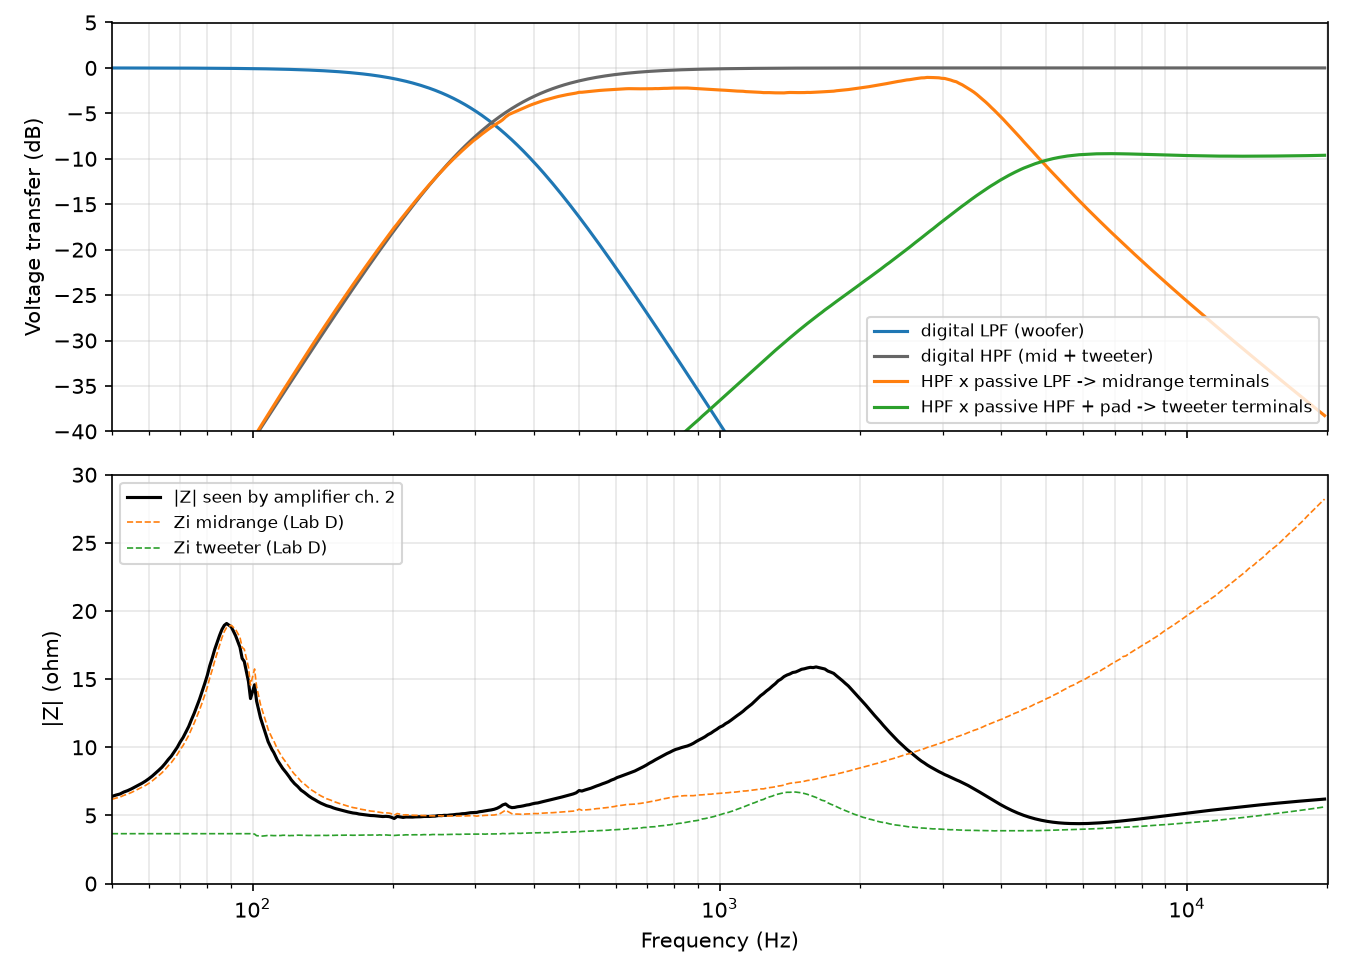
\includegraphics[width=0.88\linewidth]{xover_filters.png}
\caption{Top: voltage at each driver's terminals per volt in, from the digital filters (blue, grey)
and after the passive filters loaded by the real drivers (orange, green). Bottom: impedance seen by
amplifier channel~2 (black) and the two drivers' measured $Z_i$ (dashed).}\label{fig:filters}
\end{figure}

\begin{figure}[htbp]
\centering
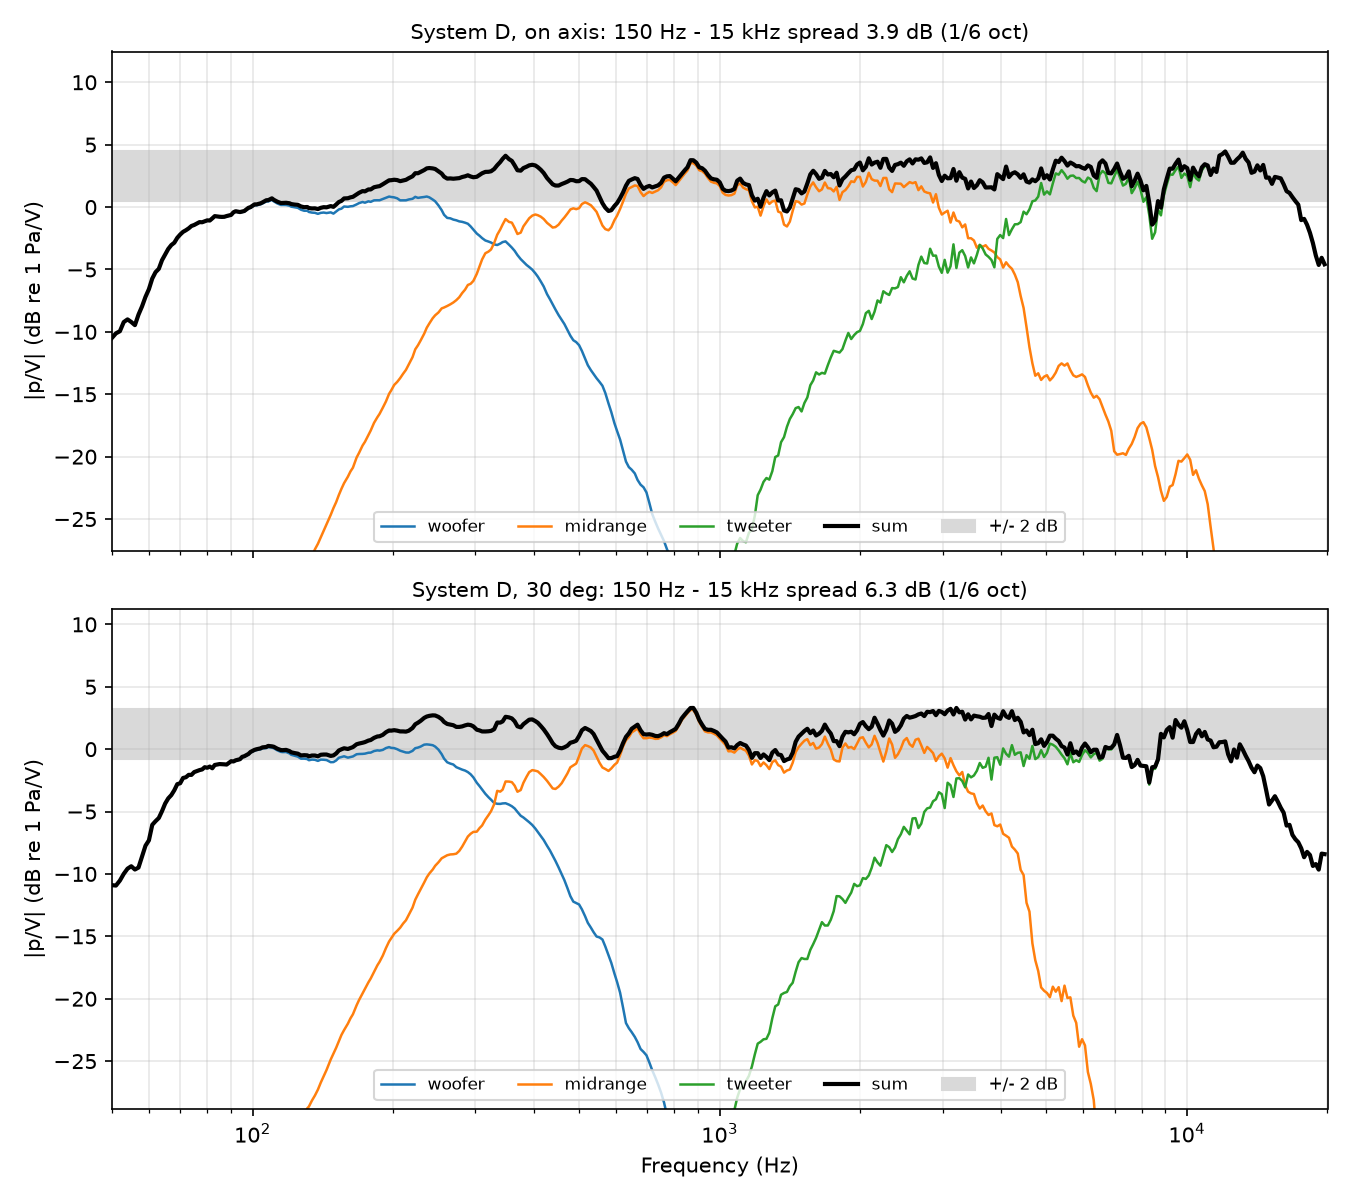
\includegraphics[width=0.88\linewidth]{xover_system.png}
\caption{Simulated sound from each driver and the sum, straight on (top) and at $30^\circ$ (bottom).
The grey band is $\pm\SI{2}{dB}$ around the average level.}\label{fig:system}
\end{figure}

\begin{figure}[htbp]
\centering
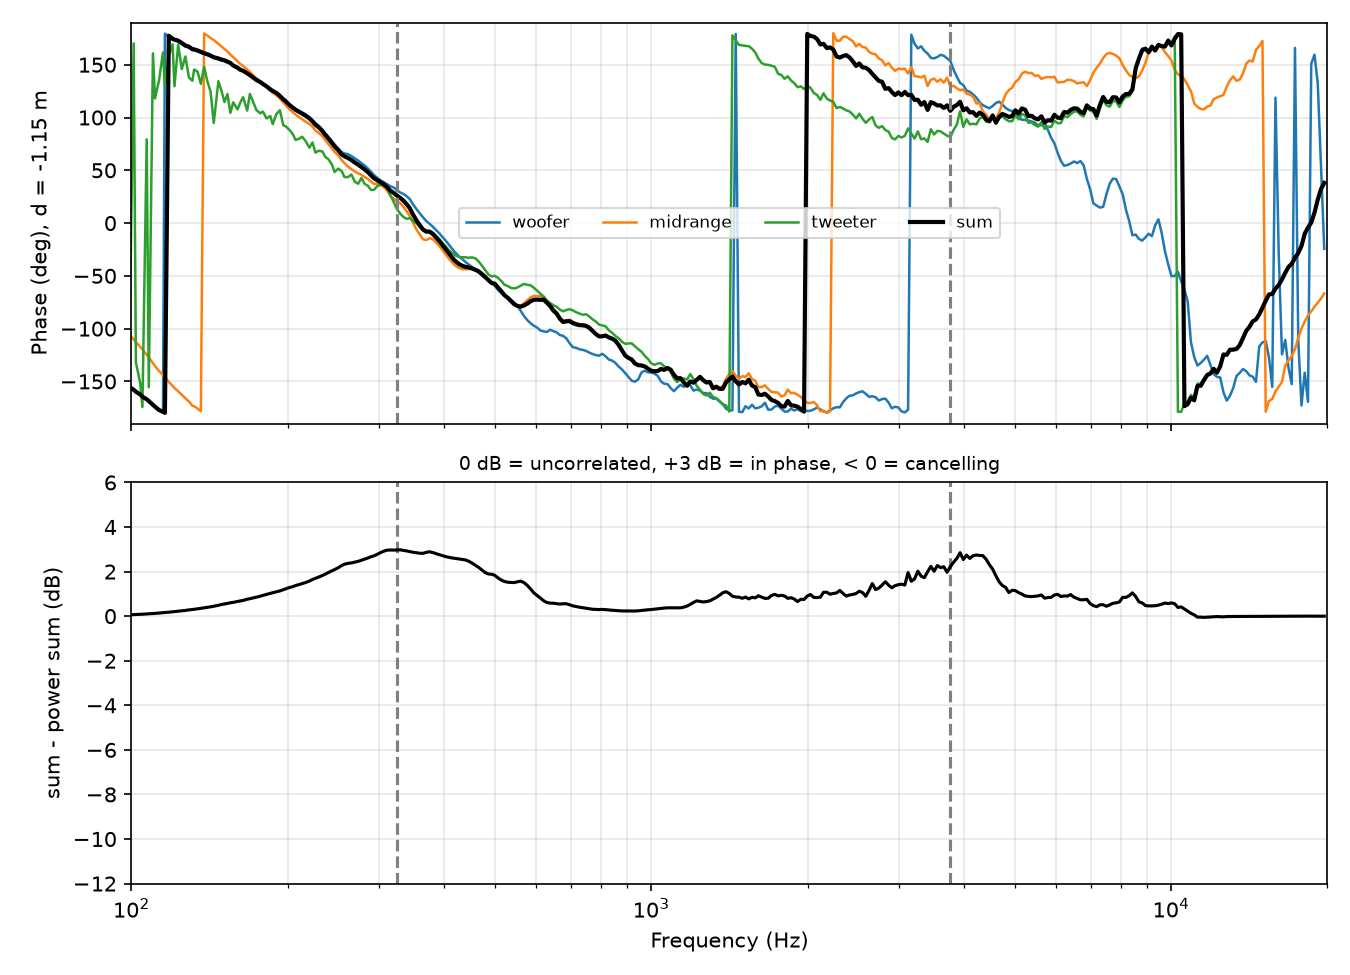
\includegraphics[width=0.88\linewidth]{xover_phase.png}
\caption{Top: phase of each driver's sound (same distance correction $d = \SI{-1.15}{m}$ for all) and of
the sum. Where two curves overlap at a crossover (dashed lines), the drivers are in phase. Bottom: the
sum compared with the power sum; $+3$\,dB at a crossover = in phase, below 0 = cancelling.}\label{fig:phase}
\end{figure}

\begin{figure}[htbp]
\centering
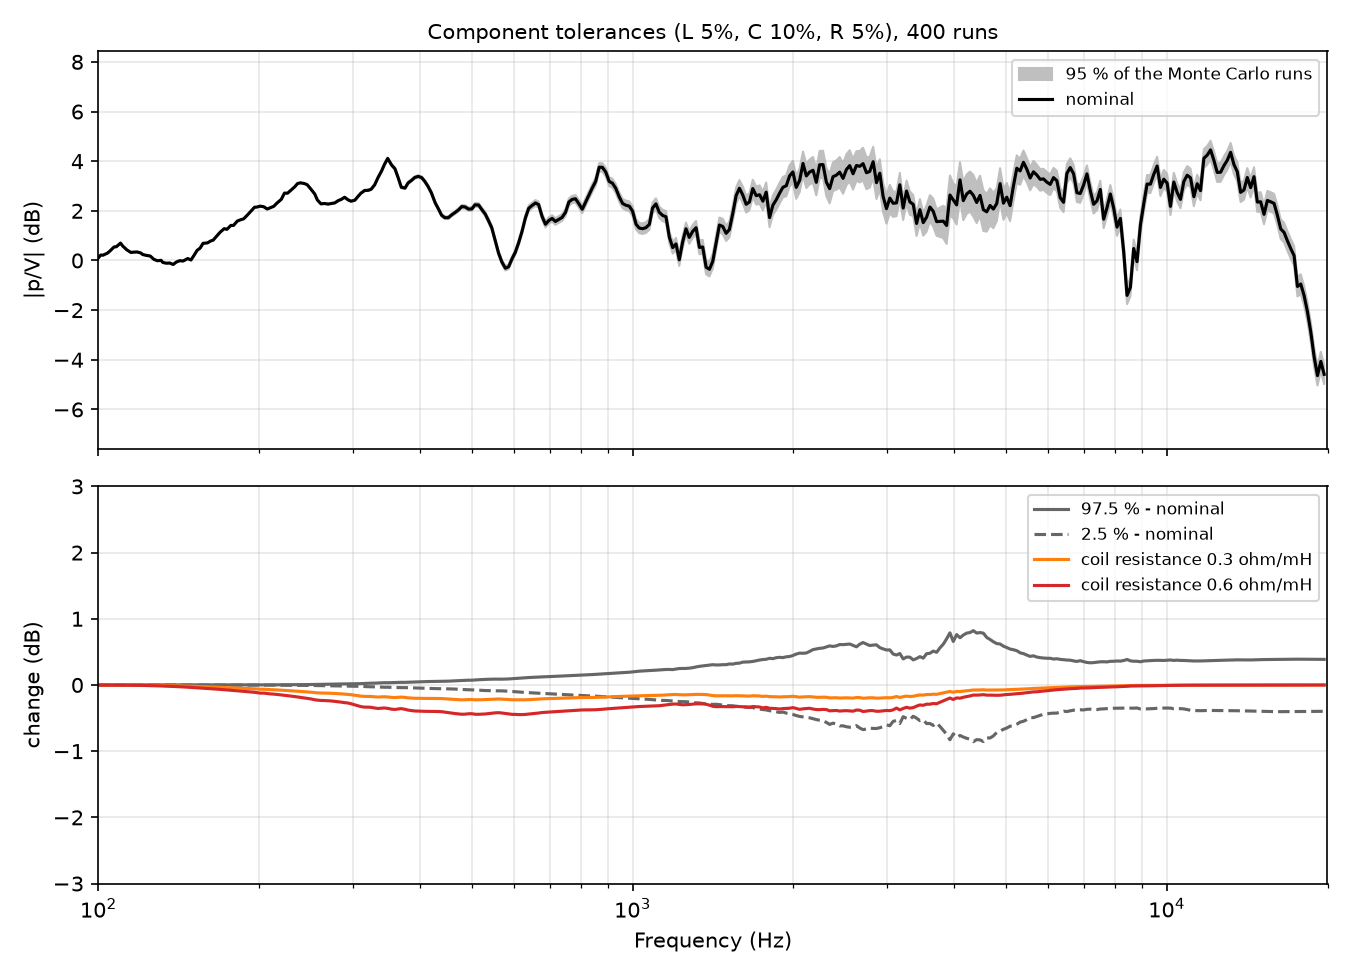
\includegraphics[width=0.88\linewidth]{xover_tolerance.png}
\caption{Top: 400 simulated boards with random part tolerances; the grey band holds 95\,\% of them.
Bottom: the same as a difference from the nominal design, plus the effect of the coils'
resistance.}\label{fig:tol}
\end{figure}

\begin{figure}[htbp]
\centering
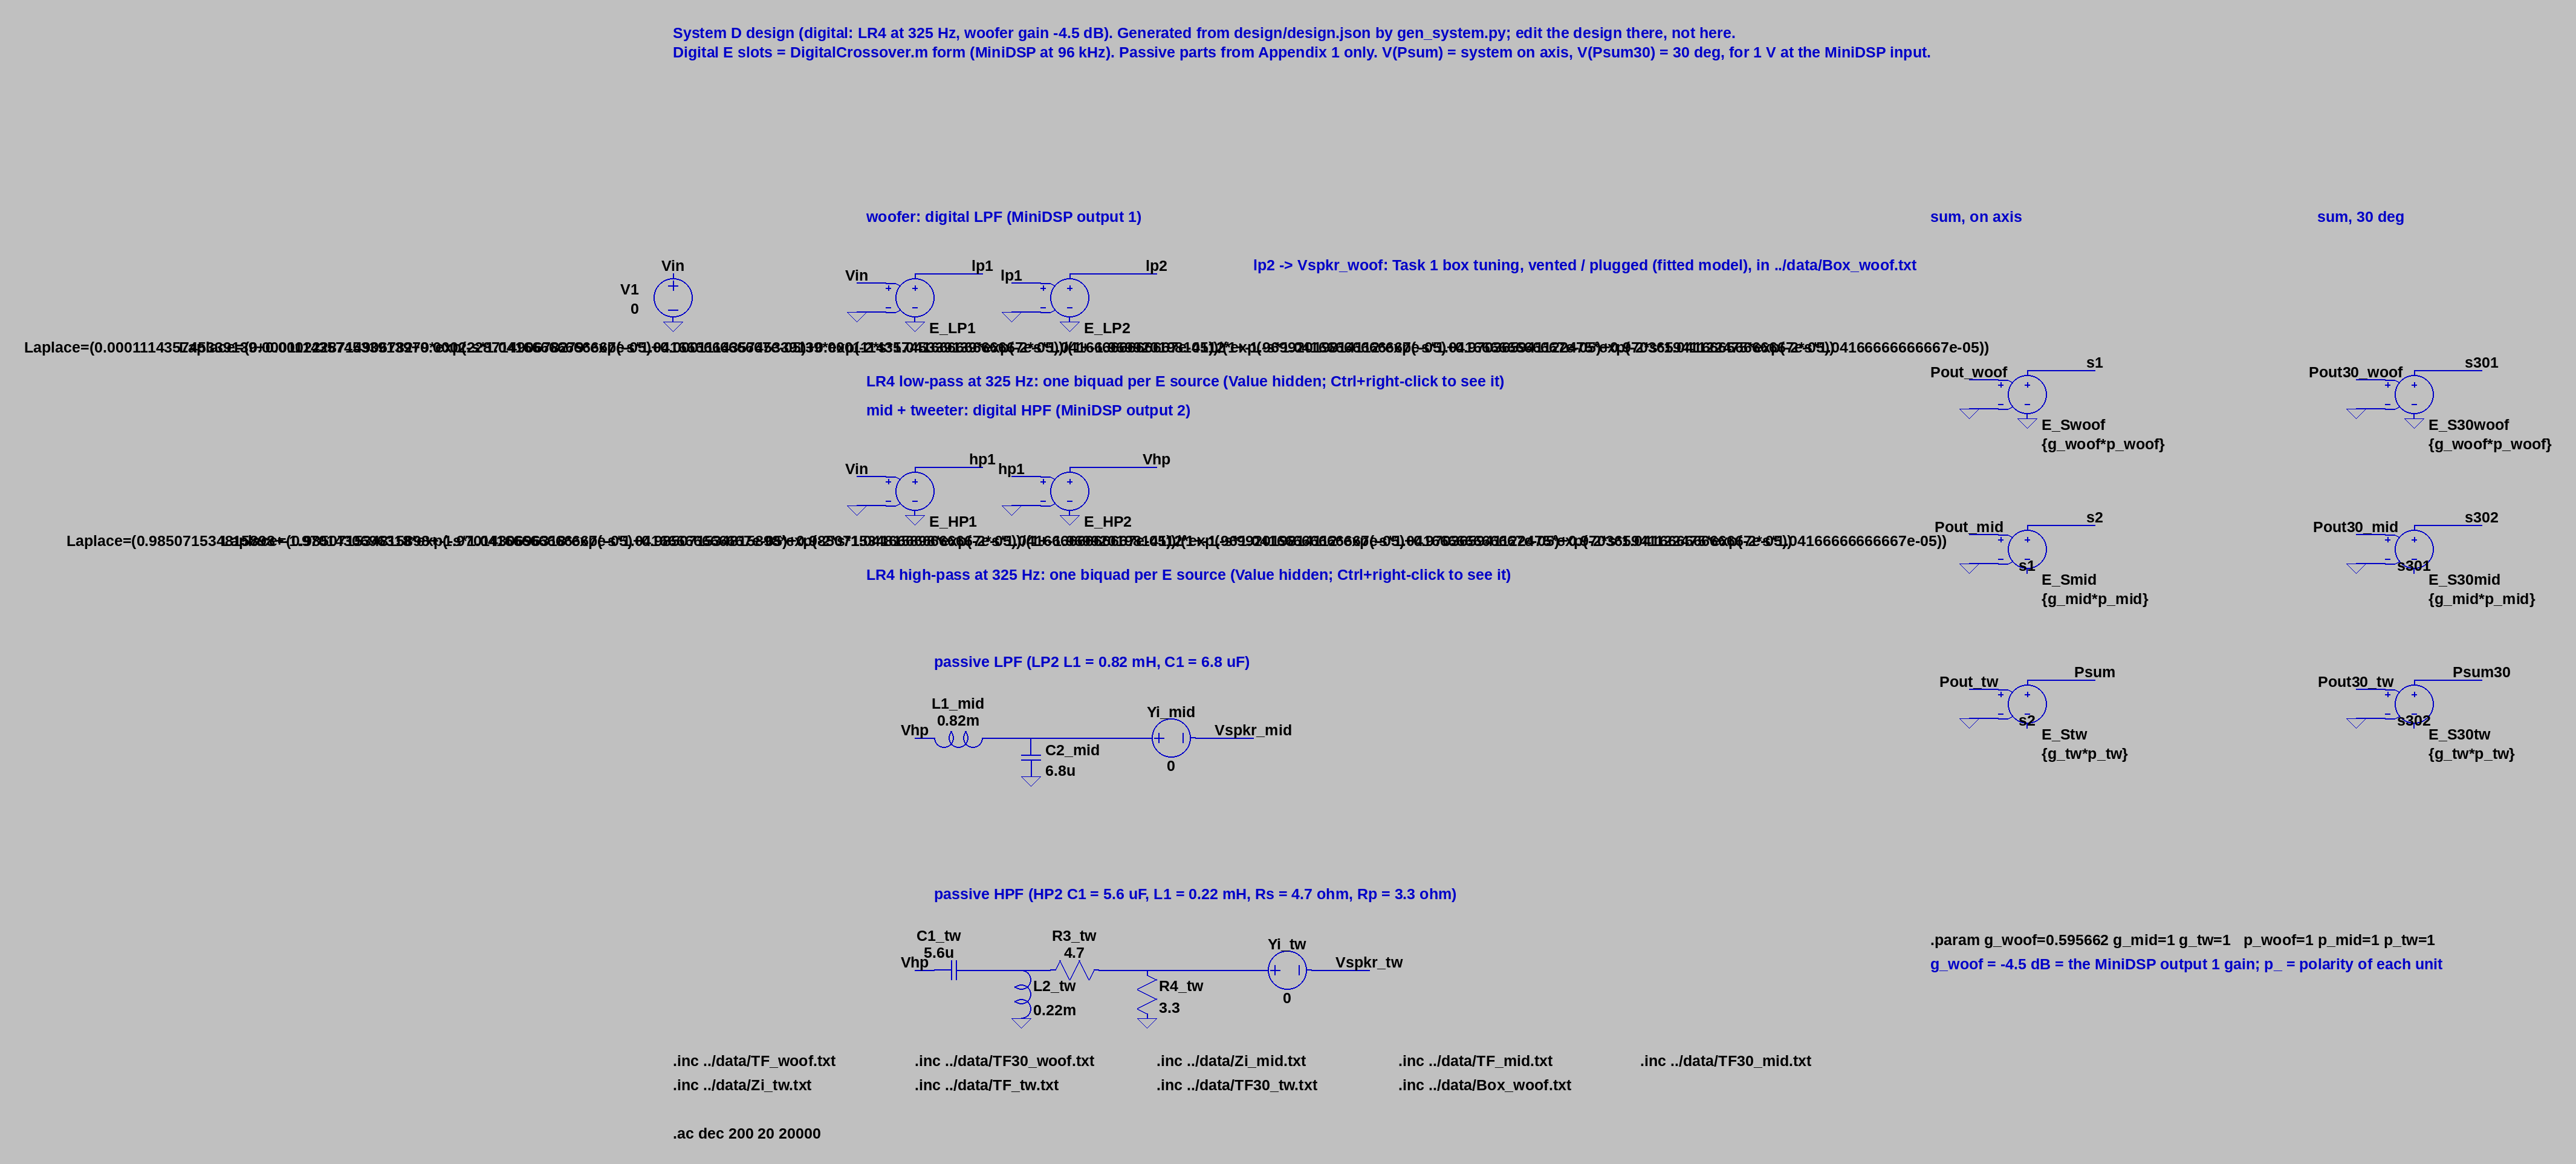
\includegraphics[width=\linewidth]{preview/System_D_design.png}
\caption{\file{ltspice/System_D_design.asc}, the complete system in LTspice. Top: the two digital
outputs, each two E sources in a row (the long \file{Laplace=} strings are hidden in LTspice; this
rendering prints them on top of each other). Middle: the passive low-pass and high-pass with L-pad,
driving the measured drivers (\file{Yi_mid}, \file{Yi_tw}). Right: the summing sources, on axis and at
$30^\circ$; \file{V(Psum)} is the system.}\label{fig:syssch}
\end{figure}

% =====================================================================================
\section{Task 3: building it}

\subsection{Setting up the MiniDSP, step by step}
The MiniDSP only needs the two LR4 filters and the woofer gain. Everything else must be switched off,
or it would add filtering we did not simulate.
\begin{enumerate}
\item Connect the MiniDSP by USB and open the MiniDSP plugin on the lab PC.
\item \textbf{Routing:} in the input/output matrix, turn on only \emph{Input~1 $\to$ Output~1} and
  \emph{Input~1 $\to$ Output~2}. All other routes off.
\item \textbf{Bypass everything except the crossover} on both outputs: PEQ, compressor and FIR set to
  bypass, only \emph{Xover} active. Leave the polarity/invert buttons off; our polarities are all normal.
\item \textbf{Output~1 (woofer):} Outputs $\to$ Output~1 $\to$ Xover $\to$ \emph{Advanced}. Paste
  the text below (it is in \file{data/dsp/MiniDSP_woofer_out1.txt}) and press \emph{Process}. These
  are two identical low-pass biquads at \SI{\xfcDig}{Hz}, which together are the LR4.
\verbfile{MiniDSP_woofer_out1.txt}
\item \textbf{Output~2 (midrange + tweeter):} the same for Output~2 with the high-pass text
  (\file{data/dsp/MiniDSP_midtw_out2.txt}):
\verbfile{MiniDSP_midtw_out2.txt}
\item \textbf{Gains:} Output~1 \SI{\xgWoof}{dB}, Output~2 \SI{0}{dB}. Input gain so the
  amplifier does not clip.
\item Save the configuration on the MiniDSP and in a file, so the demonstration on 3~Dec starts from
  the same settings.
\end{enumerate}

\textbf{Reading the numbers.} The MiniDSP's \file{a1}, \file{a2} carry the opposite sign of the
textbook form (it adds the old outputs, as in the equation in Section~\ref{sec:dsp}). That is why
\cmd{a1 = 1.9699} here, while the LTspice string in \file{data/dsp/LTspice_*.txt} has $-1.9699$.
Both are the same filter. The numbers only work at \SI{96}{kHz}: at another sample rate the same
coefficients would put the crossover somewhere else. If the design changes, rerun
\cmd{python3 xover.py --export} (or \file{DigitalCrossover(f0,'LPF',2)} in MATLAB, pasted twice) and
paste the new text.

\textbf{Quick check after setting it up:} play a sine at \SI{\xfcDig}{Hz} and measure Output~1 and
Output~2 with the oscilloscope. Both should be about \SI{6}{dB} below the input (Output~1 a further
\SI{4.5}{dB} lower), and the two should be in phase.

\subsection{The passive filter board}
Figure~\ref{fig:xcircuit} is the circuit to build. All values are single parts from the course basket
(Appendix~1 of the guide); we are not allowed to combine parts to get in-between values.
\begin{center}
\begin{tabular}{llll}
\toprule
Branch & Part & Value & Where it goes \\
\midrule
Midrange & coil & \xMidLa & in series, from amplifier $+$ to the midrange $+$ \\
Midrange & capacitor & \xMidCa & across the midrange ($+$ to $-$) \\
Tweeter & capacitor & \xTwCa & in series, from amplifier $+$ \\
Tweeter & coil & \xTwLa & from after the capacitor to ground \\
Tweeter & resistor $R_s$ & \xTwRs & in series, after that node \\
Tweeter & resistor $R_p$ & \xTwRp & across the tweeter ($+$ to $-$) \\
\bottomrule
\end{tabular}
\end{center}
Both branches start at amplifier channel~2. Wire both drivers red to $+$. Keep the two coils apart and
at right angles to each other, so one does not pick up the other's field.
\todo{photo of the board, actual parts used, measured values if an LCR meter is available.}

\subsection{Measuring the complete system}
Plan for the anechoic chamber (vents covered; the chamber cannot measure below \SI{125}{Hz} anyway):
\begin{enumerate}
\item Each driver alone through its whole chain (MiniDSP active, the other output muted). Compare with
  the single-driver curves in Figure~\ref{fig:system}. If one is off, the fault is in that branch.
\item All three together, $0^\circ$ and $30^\circ$. Compare with the sum.
\item Flip the woofer's wires: there must be a deep dip at \SI{\xxWM}{Hz}. Flip the tweeter: a dip at
  \SI{\xxMT}{Hz}. A deep dip proves the drivers really are in phase there with normal wiring, so this
  checks both the wiring and our phase model.
\end{enumerate}
\todo{measured vs.\ simulated, and what we changed.}

% =====================================================================================
\section{Task 4: listening test}
In the IEC 60268-13 listening room (Lecture~10), planned:
\begin{itemize}
\item \textbf{Set-up:} the box at the standard position, the listener \SI{2.5}{m} away straight in
  front, ears at about tweeter height. Level set to \SI{80}{dB(A)} on pink noise with a sound level
  meter, so ``louder'' does not win by default.
\item \textbf{Comparison:} A/B pairs. A = our design, B = one change (woofer gain $\pm\SI{2}{dB}$,
  tweeter $R_s$ one value up or down, vent plugged vs.\ open). The operator switches; the listener
  does not know which is which. Every pair is played twice, in both orders.
\item \textbf{Music:} 20--30\,s clips with a male voice, acoustic guitar or piano, steady bass, and
  pink noise.
\item \textbf{Questions:} per clip, which one they prefer (A, B or no difference), and 1--5 for amount
  of bass, natural voices, brightness, and overall. Free comments.
\item \textbf{Listeners:} at least 6, including people outside the group, after a short practice
  round.
\end{itemize}
\todo{results (count preferences, average scores per question) and what we changed because of them.}

\section{Conclusion}
\todo{after Tasks 3 and 4: final design, measured vs.\ simulated, what we would change.}

% =====================================================================================
\appendix
\section{Files}
Everything lives in \cmd{Project/Final design/} (the export of the raw lab data is in
\file{Project/matlab/export_systemD.m}).
\begin{center}
\begin{tabularx}{\linewidth}{lX}
\toprule
File & What it is \\
\midrule
\file{design/design.json} & the design: every value in this document \\
\file{design/xover.py} & the whole system in Python; \file{--plots} makes the Task 2 figures, \file{--export} the MiniDSP text \\
\file{ltspice/task1/box_model.py} & the Task 1 fit and the tuning table; \file{--plots} makes the Task 1 figures \\
\file{ltspice/task1/Task1_WooferBox.asc} & the woofer box in LTspice (made by \file{gen_box_ltspice.py}) \\
\file{ltspice/System_D_design.asc} & the complete system in LTspice (made by \file{gen_system.py}) \\
\file{ltspice/units/} & each driver alone with its measured data, no filter \\
\file{data/} & the LTspice data files, \file{csv/} the same data for the scripts, \file{dsp/} the filter text \\
\file{app/index.html} & Crossover Studio: change any value and see the response, in the browser \\
\bottomrule
\end{tabularx}
\end{center}
The \file{.asc} files are generated: change \file{design.json} or the scripts and rerun them rather
than editing the schematics by hand. \file{--verify} on either generator runs LTspice and compares it
with the Python model.

\end{document}
